\documentclass[a4paper]{article}

\usepackage{amsmath}
\usepackage{amsfonts}
\usepackage{amsthm}
\usepackage{dynkin-diagrams}
\usepackage{algorithm2e}
\usepackage{enumerate}
\usepackage{tikz}

\usetikzlibrary{knots, cd}

\newtheorem{theorem}{Theorem}[section]
\newtheorem{corollary}[theorem]{Corollary}
\newtheorem{lemma}[theorem]{Lemma}
\newtheorem{question}[theorem]{Question}
\newtheorem{proposition}[theorem]{Proposition}
\newtheorem{problem}[theorem]{Problem}
\newtheorem{conjecture}[theorem]{Conjecture}

\theoremstyle{definition}
\newtheorem{examples}[theorem]{Examples}
\newtheorem{example}[theorem]{Example}
\newtheorem{notation}[theorem]{Notation}


\begin{document}

\RestyleAlgo{boxruled}

\begin{titlepage}
\begin{center}
\pagenumbering{gobble}
\Large{Department of Mathematics \\ of the University of Bern}\\
\vspace*{3.5cm}
\Huge{\textbf{Coxeter Quotients \\ of Link Groups}}\\
\vspace*{6.5cm}
\Large{Master Thesis of} \\ \Large{\textbf{Levi Ryffel}}\\
\vspace*{.25cm}
Supervised by \\ \textbf{Prof. Dr. Sebastian Baader}\\
\vspace*{2cm}
February 2020
\end{center}
\end{titlepage}
\pagenumbering{arabic}

\tableofcontents
\newpage

\section*{Introduction}

\newpage
\section{Consequences of Coxeter Quotients}
The knot group $\pi(K)$ is a very fine invariant of knots, in that it distinguishes basically all inequivalent knots \cite[Corollary 2.1]{gordon1989}. This comes with the tradeoff that presentations of groups, i.e., the form in which knot groups are most frequently given, are very difficult to handle.

One possible compromise for this is to instead study quotients of the knot group. One traditional candidate, the abelianisiation $\pi(K)^{\text{ab}}$ of the knot group, fails horribly: for any knot $K \subset S^3$ we have that $\pi(K)^{\text{ab}}$ is isomorphic to the integers: see Appendix \ref{subsubsec:the_knot_group}. In other words, there is no information whatsoever about the knot in the abelianisation of its knot group.

In this section we present a different sort of quotients of the knot group, namely Coxeter quotients.

\subsection{Coxeter Quotients}
Let $L \subset S^3$ be a link. A \textit{Coxeter quotient} is a quotient $\pi(K)/N$ of the link group which is isomorphic to a Coxeter group $W(M)$ such that every meridian in $\pi(L)$ corresponds to a reflection in $W(M)$.

In many cases, finding Coxeter quotients of links is rather straight-forward, at least with the help of a computer. This is because checking whether a specific set of Coxeter relations induces a Coxeter quotient of a link amounts to checking the validity of the defining relations in its link group. More information on this can be found in Appendix \ref{subsec:coxeter_quotients_algorithms}.


\subsection{The Reflection Quotient}\label{subsec:reflection-quotient}
The \textit{reflection quotient} is the group $r(L) = \pi_1(S^3 \setminus L) / \langle \langle m^2 \rangle \rangle$, where $m$ is any meridian of $L$. Coxeter quotients of a link $L$ are also quotients of $r(L)$. The fact justifying the study of quotients of $r(K)$ lies in the following theorem.

\begin{theorem}[Boileau-Zimmermann \cite{boileau1989}, Theorem 1]
Let $K$ and $K'$ be knots such that $r(K)$ and $r(K')$ are infinite. Then $K$ and $K'$ are equivalent if and only if $r(K)$ and $r(K')$ are isomorphic.
\end{theorem}

It is easy to write down a presentation of the reflection quotient from a presentation of the link group $\pi(L) = \langle S \; | \; R \rangle$ of a link $L \subset S^3$. Just add the relations $s^2$ for all $s \in S$, and simplify $R$ by replacing all occurrences of $s^{-1}$ by $s$ and all occurrences of $s^2$ by the empty word. These presentations are generally shorter, easier to read and less prone to mistakes since it is no longer possible to confuse meridians with their inverses.

Note in addition that the Wirtinger algorithm (see section \ref{subsubsec:the_knot_group}) can be simplified so that the relation $ca = ab$ in Figure \ref{fig:wirtinger-relations} reads $acab = 1$ in the reflection quotient.
For these reasons, we will now mainly consider the reflection quotient instead of the link group.

\subsection{The Meridional Rank Conjecture}
For a link $L \subset S^3$ we define its \textit{Coxeter rank}, abbreviated $\text{cr } L$, to be the maximal number $n$ such that $L$ has a Coxeter quotient of rank $n$. Abbreviating the meridional rank of $L$ by $\text{mr }L$ and the bridge index of $L$ by $\text{bi } L$, we have the following.

\begin{theorem}
Let $L \subset S^3$ be any link. Then we have the following chain of inequalities: $\textup{cr }L \leq \textup{mr }L \leq \textup{bi } L$.
\end{theorem}

\begin{proof}
The inequality $\textup{mr } L \leq \text{bi } L$ is well-known. Moreover, $\text{bi } L \leq \text{mr } L$, is a direct consequence of \cite[Lemma 2.1]{felikson2009}.
\end{proof}

Let us refer to a link $L \subset S^3$ that has a Coxeter quotient of rank $\text{bi } L$ as a \textit{Coxeter link}. Then we immadiately obtain:

\begin{corollary}\label{cor:coxeter-links-meridional-rank}
Coxeter links satisfy the meridional rank conjecture.
\end{corollary}

\subsection{The Meridional Rank of Connected Sums}

\begin{theorem}\label{thm:connected-sums-coxeter-rank}
Let $K$ and $K'$ be knots. Then $\textup{cr } K\#K' \geq \textup{cr } K + \textup{cr } K' - 1$.
\end{theorem}

\begin{proof}
Let $W$ and $W'$ be Coxeter quotients of $K$ and $K'$, respectively. First we choose diagrams of $K$ and $K'$ such that the generators of $\pi(K)$ and $\pi(K')$ that get mapped to generating reflections of $W$ and $W'$ are diagram meridians. Let $s \in \pi(K)$ and $s' \in \pi(K')$ each be one of those diagram meridians.

Now observe that $\pi(K\#K')$ is of the form $\pi(K) * \pi(K') / ss'$. Thus, we can explicitly write down a Coxeter quotient of $K\#K'$ as follows. Let $\Gamma$ and $\Gamma'$ be the Coxeter graphs associated to $W$ and $W'$. Then there is a Coxeter quotient of $K\#K'$ with graph
\begin{center}
\begin{tikzpicture}
\draw[dashed] (0.85, 0.15) -- (0.15, 0.85);
\draw[dashed] (-0.15, 0.85) -- (-0.85, 0.15);
\draw (0.8, 0) -- (-0.8, 0);

\node at (0, 1) {$s$};
\node at (-1, 0) {$\Gamma$};
\node at (1, 0) {$\Gamma'$};
\node at (0, 0.2) {$\infty$};
\end{tikzpicture}
\end{center}
which has rank $\text{rk } W + \text{rk } W' - 1$. 
\end{proof}

\begin{corollary}
Knots of Coxeter rank two are prime.
\end{corollary}

\begin{proof}
This follows directly from the facts that bridge index one knots are prime and that the bridge index satisfies the same inequality, see Proposition \ref{prop:bridge-index-connected-sum}.
\end{proof}

\begin{corollary}
There are knots of arbitrarily high meridional rank.
\end{corollary}

\begin{proof}
Just take connected sums of your favorite non-trivial knot.
\end{proof}

\begin{corollary}
Connected sums of Coxeter knots are Coxeter knots.
\end{corollary}

\begin{proof}
Let $J, K \subset S^3$ be arbitrary knots. Then we have already shown that $\text{bi } J\#K = \text{bi } J + \text{bi } K - 1$ and $\text{cr } J\#K \leq \text{bi } J\#K$. If $J$ and $K$ are both Coxeter knots then equality immediately follows from Theorem \ref{thm:connected-sums-coxeter-rank}.
\end{proof}

\newpage

\section{Existence of Coxeter Quotients}
This section describes methods for finding Coxeter quotients and particular examples. The gist of it is as follows. Let $L \subset S^3$ be a link, and let $\pi(L) = \langle S \; | \; R \rangle$ be a presentation of its knot group, where $S$ consists of meridians. If we can interpret the meridians $S$ as reflections in a Coxeter group $W$ generated by $S$ such that all the relations $R$ are satisfied in $W$, then $\pi(L)$ admits a Coxeter quotient isomorphic to $W$.

\begin{example}[The Knot $8_5$]
Consider $K = 8_5$ from Rolfsen's knot table, compare Figure \ref{fig:8-5}. Then $K$ has a Coxeter quotient with graph $$A_3 = \dynkin[Coxeter]{A}{3}$$ which is isomorphic to the permutation group $S_3$.

\begin{figure}[ht]
\centering
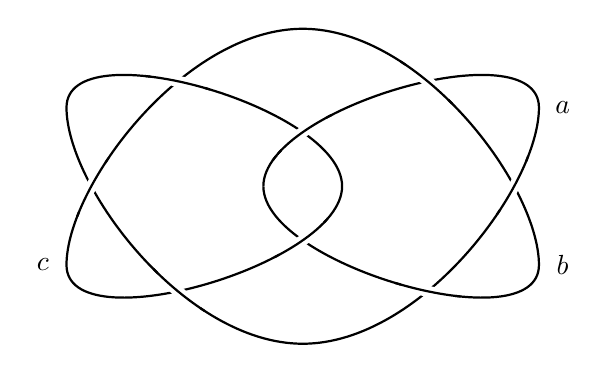
\begin{tikzpicture}
\begin{knot}[consider self intersections = true, clip width = 5, ignore endpoint intersections=false,
%draft mode = crossings,
flip crossing/.list={3, 5, 7}]
\strand[thick] (-0.5, 0) .. controls +(0, 1) and +(0, 1) .. (3, 1) .. controls +(0, -1) and +(1.5, 0) .. (0, -2) .. controls +(-1.5, 0) and +(0, -1) .. (-3, 1) .. controls +(0, 1) and +(0, 1) .. (0.5, 0) .. controls +(0, -1) and +(0, -1) .. (-3, -1) .. controls +(0, 1) and +(-1.5, 0) .. (0, 2) .. controls +(1.5, 0) and +(0, 1) .. (3, -1) .. controls +(0, -1) and +(0, -1) .. (-0.5, 0);
\end{knot}

\node at (3.3, 1) {$a$};
\node at (3.3, -1) {$b$};
\node at (-3.3, -1) {$c$};
\end{tikzpicture}
\caption{The knot $8_5$}
\label{fig:8-5}
\end{figure}

Note that by the Wirtinger algorithm, the reflection quotient (defined in Section \ref{subsec:reflection-quotient}) has a presentation
$$r(8_5) = \langle a, b, c\; | \; a^2, b^2, c^2, babc(ba)^2bc(ba)^4, babc(ba)^4cbabc(ab)^2a \rangle.$$
%TODO check this
These relations are satisfied in the Coxeter group
$$W = \langle a, b, c \; | \; a^2, b^2, c^2, (ab)^2, (ac)^3, (bc)^3 \rangle.$$
Thus, $W$ is a quotient of $\pi_1(S^3 \setminus 8_5)$.
\end{example}

Note that there exist presentations of the knot $8_5$, for example, any presentation involving more than three meridians, such that the above method does not work. It is thus difficult to prove in general that a fixed link $L$ does not admit a Coxeter quotient isomorphic to a specific Coxeter group $W$.

\subsection{In 2-Bridge Knots}
This section illustrates our later strategies in a particularly easy setting, namely the 2-bridge knots, see Appendix \ref{subsubsec:bridge-index}.
\begin{theorem}
2-bridge knots are Coxeter.
\end{theorem}

\begin{proof}
2-Bridge Knots have a dihedral reflection quotient, which is itself a Coxeter group.
\end{proof}


\subsection{In Pretzel Links}
\begin{theorem}\label{thm:pretzel-links-are-coxeter}
Pretzel links are Coxeter. 
\end{theorem}

\begin{proof} First consider the situation of how assigning letters to meridians propagates in 2-braids in Figure \ref{fig:elementary-twists}.
\begin{figure}[ht]
\centering
\begin{minipage}{.5\textwidth}
\centering

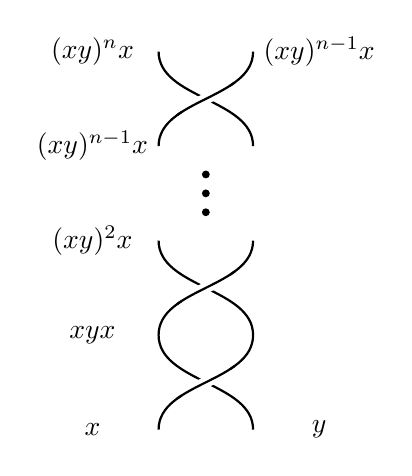
\begin{tikzpicture}[scale = 0.6]
\begin{knot}[clip width = 5, flip crossing = 2]

\strand[black, thick] (0, 0) .. controls +(0, 1) and +(0, -1) .. (2, 2) .. controls +(0, 1) and +(0, -1) .. (0, 4);

\strand[black, thick] (2, 0) .. controls +(0, 1) and +(0, -1) .. (0, 2) .. controls +(0, 1) and +(0, -1) .. (2, 4);

\strand[black, thick] (0, 6) .. controls +(0, 1) and +(0, -1) .. (2, 8);

\strand[black, thick] (2, 6) .. controls +(0, 1) and +(0, -1) .. (0, 8);

\end{knot}

\node at (1, 4.6) [circle, fill, inner sep=1pt]{};
\node at (1, 5) [circle, fill, inner sep=1pt]{};
\node at (1, 5.4) [circle, fill, inner sep=1pt]{};


\node at (-1.4, 0) {$x$};
\node at (3.4, 0) {$y$};
\node at (-1.4, 2) {$xyx$};
\node at (-1.4, 4) {$(xy)^2x$};
\node at (-1.4, 6) {$(xy)^{n-1}x$};
\node at (-1.4, 8) {$(xy)^nx$};
\node at (3.4, 8) {$(xy)^{n-1}x$};

\end{tikzpicture}

\end{minipage}%
\begin{minipage}{.5\textwidth}
\centering
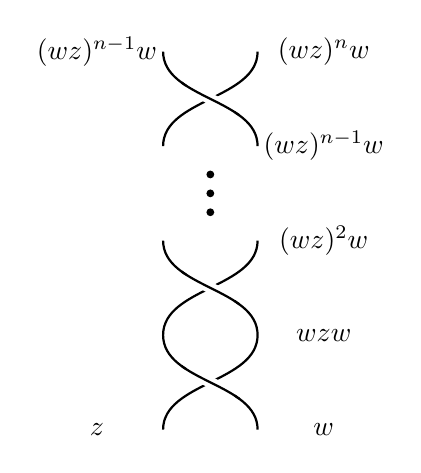
\begin{tikzpicture}[scale = 0.6]
\begin{knot}[clip width = 5, flip crossing/.list = {1, 3}]

\strand[black, thick] (0, 0) .. controls +(0, 1) and +(0, -1) .. (2, 2) .. controls +(0, 1) and +(0, -1) .. (0, 4);

\strand[black, thick] (2, 0) .. controls +(0, 1) and +(0, -1) .. (0, 2) .. controls +(0, 1) and +(0, -1) .. (2, 4);


\strand[black, thick] (0, 6) .. controls +(0, 1) and +(0, -1) .. (2, 8);

\strand[black, thick] (2, 6) .. controls +(0, 1) and +(0, -1) .. (0, 8);

\end{knot}


\node at (1, 4.6) [circle, fill, inner sep=1pt]{};
\node at (1, 5) [circle, fill, inner sep=1pt]{};
\node at (1, 5.4) [circle, fill, inner sep=1pt]{};

\node at(-1.4, 0) {$z$};
\node at(3.4, 0) {$w$};
\node at (3.4, 2) {$wzw$};
\node at (3.4, 4) {$(wz)^2w$};
\node at (3.4, 6) {$(wz)^{n-1}w$};
\node at (3.4, 8) {$(wz)^n w$};
\node at (-1.4, 8) {$(wz)^{n-1}w$};

\end{tikzpicture}

\end{minipage}
\caption{The relations for 2-braids}
\label{fig:elementary-twists}
\end{figure}

Now note that assigning letters of meridians as in the local situation in Figure \ref{fig:local-picture-pretzel-link}, we in fact obtain a generating set of the link group $\pi(P(l_1, \dots, l_k))$.


\begin{figure}[ht]
\centering
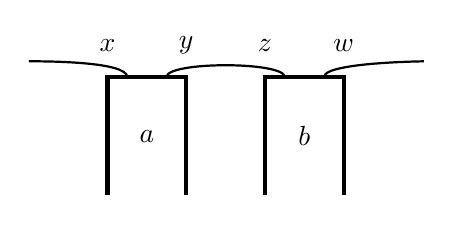
\begin{tikzpicture}
\draw[ultra thick] (0, -1.5) -- (0, 0) -- (1, 0) -- (1, -1.5);
\draw[ultra thick] (2, -1.5) -- (2, 0) -- (3, 0) -- (3, -1.5);

\begin{knot}
\strand[thick] (0.25, 0) .. controls +(0, 0.2) and +(0.2, 0) .. (-1, 0.2);
\strand[thick] (0.75, 0) .. controls +(0, 0.2) and +(0, 0.2) .. (2.25, 0);
\strand[thick] (2.75, 0) .. controls +(0, 0.2) and +(0.2, 0) .. (4, 0.2);
\end{knot}

\node at (0, 0.4) {$x$};
\node at (1, 0.4) {$y$};
\node at (2, 0.4) {$z$};
\node at (3, 0.4) {$w$};

\node at (0.5, -0.75) {$a$};
\node at (2.5, -0.75) {$b$};
\end{tikzpicture}

\caption{A local picture}
\label{fig:local-picture-pretzel-link}
\end{figure}

Putting these 2-braids together as in Figure \ref{fig:local-picture-pretzel-link} we obtain the following relation in the knot group from the requirement that $y = z$ according as to whether $a$ and $b$ are positive or negative:

\begin{itemize}
\item If both $a$ and $b$ are positive, then we obtain $(xy)^{a-1}x = (yw)^by.$
\item If $a$ is positive and $b$ is negative, we obtain $(xy)^{a-1}x = (wy)^{-b+1}w$.
\item If $a$ is negative and $b$ is positive, we obtain $(yx)^{-a}y = (yw)^b y$.
\item If both $a$ and $b$ are negative, then we obtain $(yx)^{-a}y = (wy)^{-b+1}w$.
\end{itemize}

All these relations follow from the Coxeter relations $(xy)^{|a|} = (yw)^{|b|} = 1$. Assigning generators as in Figure \ref{fig:local-picture-pretzel-link} we get a quotient of the desired form.
\end{proof}

This Theorem and its proof have some consequences that, although well-known, still require some work to prove. So it is worth it to state them with proofs in our setting.

\begin{corollary}
Pretzel links satisfy the meridional rank conjecture.
\end{corollary}

\begin{proof}
This is just Corollary \ref{cor:coxeter-links-meridional-rank}.
\end{proof}

%TODO
\begin{question}
Is there more to deduce?
\end{question}

It might be worth pointing out that the explicit Coxeter quotient obtained is described by the matrix

$$
\renewcommand\arraystretch{1.2}
M = \left( \begin{matrix}
1 & l_1 & \infty & \cdots & \cdots &\cdots & \infty & l_n \\
l_1 & 1 & l_2 & \infty & \cdots & \cdots & \infty & \infty \\
\infty & l_2 & 1 & l_3 & \infty &\cdots & \infty & \infty \\
\vdots & \infty  & l_3 & 1 & \ddots & \ddots & \vdots & \vdots \\
\vdots & \vdots & \infty & \ddots & \ddots & \ddots & \infty & \vdots \\
\vdots & \vdots & \vdots & \ddots &\ddots & 1 & \l_{n-2} & \infty \\
\infty & \infty & \infty & \cdots & \infty & l_{n-2} & 1 & l_{n-1} \\
l_n & \infty & \infty & \cdots & \cdots & \infty  & l_{n-1} & 1
\end{matrix} \right).$$

\subsection{In Torus Links}
I conjecture that the Torus links $T(n, n+1)$ have Coxeter quotients isomorphic to $S_{n+1}$ which is isomorphic to a Coxeter group of rank $n$. Use some presentation constructed using the twist relations in Figure \ref{fig:twist-relations}. Most likely success will come from choosing the first $n$ left-most generators.

\begin{figure}[ht]
\centering
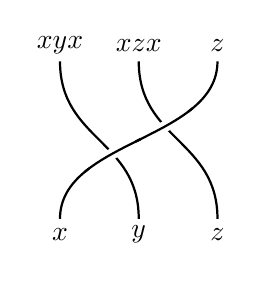
\begin{tikzpicture}
\begin{knot}[clip width = 5, consider self intersections = true]


\strand[black, thick] (0,0) .. controls +(0, 1) and +(0, -1) .. (2,2);

\strand[black, thick] (1, 0) .. controls +(0,1) and +(0, -1) .. (0, 2);

\strand[black, thick] (2, 0) .. controls +(0, 1) and +(0, -1) .. (1,2);


\node at (0, -0.2) {$x$};
\node at (1, -0.2) {$y$};
\node at (2, -0.2) {$z$};

\node at (0, 2.2) {$xyx$};
\node at (1, 2.2) {$xzx$};
\node at (2, 2.2) {$z$};

\end{knot}
\end{tikzpicture}
\caption{The twist relation in the case $n = 3$}
\label{fig:twist-relations}
\end{figure}

\begin{example}[The $(3, 7)$-Torus Knot]
The $(3, 7)$-torus knot $T(3,7)$ is an example of a knot $K$ satisfying the strict inequality $\text{cr } K < \text{bi } K$. In fact, $\text{cr } K = 1$. There three things that go into this. First, the determinant of $K$ is one. Since the existence of a nontrivial Fox $n$-coloring (i.e., a rank two Coxeter quotient) implies that $n$ divides the determinant of $K$, we immediately get that $K$ has no Coxeter quotient of rank two.

Secondly, by brute force we find that $K$ does not admit any finite rank three quotient. This is actually not hard to check since the only finite irreducible Coxeter groups with abelianization $\mathbb{Z}/2\mathbb{Z}$ of rank three are just $S_4$ and the icosahedral group.

Finally, recall that the center of $\pi(K)$ is generated by the element $a^3 = b^7$, where $a$ and $b$ are both a composition of an odd number of meridians. Since they have to be mapped to the center of any Coxeter group, any Coxeter quotient of $K$ would need to have nontrivial center. But by Corollary 1.3 in \cite{hosaka2005}, all such Coxeter groups are reducible or finite.
\end{example}

This example disproves the fact that equality $\text{cr } L = \text{bi } L$ holds for any link. Summarizing this, we obtain the following.

\begin{proposition}
There exists a link $L \subset S^3$ satisfying $\text{cr } L < \text{bi } L$.
\end{proposition}

\subsection{In Positive Braids (?)}
I have no idea how this should work. But it might be fun to consider.


\newpage
\appendix
\section{Appendix}
% Everything that is not directly related to Coxeter quotients.
\subsection{Topology}
\subsubsection{Topological Spaces}
We recall some basic definitions in the theory of topological spaces.  This is not a proper introduction to the subject of topology. All the material used here can be found in \cite{lee2011} or \cite{munkres2000}. 

A \textit{topological space} is a set $X$ equipped with a notion of \textit{open subsets}, satisfying the following conditions.
\begin{enumerate}
\item The empty set $\emptyset$ and the whole set $X$ are both open.
\item For finitely many open sets $U_1, \dots, U_n$, their intersection $\bigcap_{i = 1}^n U_i$ is open.
\item For arbitrarily many open sets $\{U_i\}_{i \in I}$, their union $\bigcup_{i \in I} U_i$ is open.
\end{enumerate}
The set of all open subsets of a topological space is called its \textit{topology}.

A map $f: X \rightarrow Y$ is called \textit{continuous} if for any open subset $U \subset Y$, its preimage $f^{-1}(U) \subset X$ is open. If $f$ is continuous and bijective with continuous inverse, then we call $f$ a \textit{homeomorphism}. If there exists a homeomorphism between topological spaces $X$ and $Y$ we consider them equivalent, or \textit{homeomorphic}. Any property of topological spaces that can be described using only their points and topology is invariant under homeomorphism. This is because homeomorphisms induce structure-preserving bijections on the involved topologies.

A \textit{basis} of a topological space $X$ is a subset $\{U_i\}_{i \in I}$ of the topology of $X$ such that for any open set $U \subset X$ there exists $J \subset I$ such that $U = \bigcup_{j \in J} U_j$. A topological space that has a countable basis is called \textit{second-countable}. There is also a notion of first-countable topological spaces, but this is not particularly important for our purposes.

A \textit{neighborhood} of a set $A$ is an open set $U$ containing $A$. If $A$ consists of just a point, we also speak of neighborhoods of points.
We call a topological space $X$ \textit{Hausdorff} if for any two points $x, y \in X$ there exist disjoint neighborhoods $U$ of $x$ and $V$ of $y$.

One important class of topological spaces are the so-called \textit{manifolds}. These are precisely the topological spaces $X$ satisfying
\begin{enumerate}
\item $X$ is Hausdorff.
\item $X$ is second-countable.
\item $X$ is locally homeomorphic to $\mathbb{R}^n$ for some fixed $n$. That is, any $x \in X$ has a neighborhood $U$ such that there exists a homeomorphism $f: U \rightarrow \mathbb{R}^n$.
\end{enumerate}

We call a topological space $X$ \textit{connected} if for any two open sets $U, V \subset X$ such that $X = U \cup V$ it follows that either $U$ or $V$ is empty. Moreover, a topological space $X$ is \textit{compact}, if every open cover of $X$ admits a finite subcover.

\subsubsection{The Fundamental Group}
We briefly introduce the fundamental group $\pi_1(X)$ of a topological space $X$. For a proper introduction, consider \cite{hatcher2002}.

A \textit{path} in a topological space $X$ is a continuous map $\gamma: [0, 1] \rightarrow X$. The path $\gamma$ is called \textit{closed} if $\gamma(0) = \gamma(1)$. A \textit{path-homotopy} between paths $\gamma$ and $\gamma'$ satisfying $\gamma(0) = \gamma'(0)$ and $\gamma(1) = \gamma'(1)$ is a family of maps $H_t: [0, 1] \times [0, 1] \rightarrow X$ for $t \in [0,1]$, if
\begin{enumerate}
\item The map $(t, s) \mapsto H_t(s)$ is continuous.
\item We have that $H_0 = \gamma$ and $H_1 = \gamma'$
\item For all $t$ we have $H_t(0) = \gamma(0)$ and $H_t(1) = \gamma(1)$.
\end{enumerate}
If there exists a path-homotopy between paths $\gamma$ and $\gamma'$, we say that $\gamma$ is \textit{path-homotopic} to $\gamma'$.

As a set, the \textit{fundamental group} $\pi_1(X, x)$ of a topological space $X$ with respect to the base point $x \in X$ is the set of closed paths in $X$ up to the equivalence relation given by path-homotopy. As the name of this set suggests, there is a natural group structure on this set. This is induced by \textit{path-concatenation}, defined as
$$(\gamma \cdot \gamma') (t) = \begin{cases}
\gamma(2t) & t \leq 1/2 \\
\gamma'(2t - 1)	& t \geq 1/2.
\end{cases}$$
A proof that the fundamental group is in fact a group can be found in \cite{hatcher2002}.

Let $X$ be a \textit{path-connected} topological space, i.e., for any two points $x, y \in X$ there exists a path $\gamma$ in $X$ with $\gamma(0) = x$ and $\gamma(1) = y$. Then the two fundamental groups $\pi_1(X, x)$ and $\pi_1(X, y)$ are isomorphic via the isomorphism given by $[\beta] \mapsto [\gamma^{-1} \cdot \beta \cdot \gamma]$. Thus, we frequently talk about the fundamental group of a path-connected topological space without reference to a base point. In this situation, we denote the fundamental group by $\pi_1(X)$.

\subsubsection{Some Homology Theory}
Homology groups are introduced in \cite{hatcher2002}, in which also proofs the following theorems can be found.

\begin{theorem}[Hurewicz]
Let $X$ be a path-connected topological space. Then $H_1(X)$ is isomorphic to the abelianization $\pi_1(X)^{\textup{ab}}$ of its fundamental group.
\end{theorem}

\begin{theorem}[Alexander and Poincar\'e Duality]
Let $X$ be a compact, locally contractible subspace of $S^n$. Then, for $i \geq 1$, there is an isomorphism $$H_i(S^n \setminus X) \rightarrow H_i(X).$$
\end{theorem}
\subsection{Knot Theory}
\subsubsection{Links}
A \textit{knot} $K$ is the image of a smooth embedding of $S^1$ into $S^3$. A \textit{link} $L$ is a disjoint union of finitely many knots. Two links $L \subset S^3$ and $L' \subset S^3$ are said to be \textit{equivalent} if there exists a diffeomorphism between the pair $(S^3, L)$ and the pair $(S^3, L')$, i.e., a diffeomorphism $S^3 \rightarrow S^3$ that restricts to a diffeomorphism of the links $L \rightarrow L'$.

\begin{example}[Torus Links]
Let $p, q$ be integers. Consider the universal covering $\mathbb{R}^2 \rightarrow T^2$, where $T^2 \subset \mathbb{R}^3$ is a standardly embedded torus (consider e.g. Example 6 of Section 2-2 in \cite{docarmo1976}). Then the $(p,q)$-\textit{torus link} is the image of the lines through $\mathbb{Z}e_1$ of slope $p/q$.
\end{example}

\begin{example}[Pretzel Links]
The $(l_1, \dots, l_k)$-\textit{Pretzel link} is the link obtained by connecting 2-braids in the way indicated in Figure \ref{fig:pretzel-link}.

\begin{figure}[ht]
\centering
\begin{minipage}{0.5\textwidth}
\centering
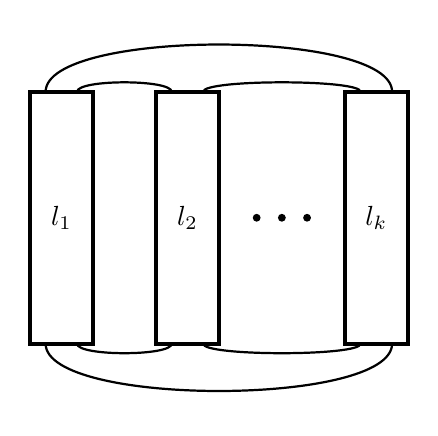
\begin{tikzpicture}[scale = 0.8]
\draw[ultra thick] (0, 0) rectangle (1,4);
\draw[ultra thick] (2, 0) rectangle (3, 4);
\node at (3.6, 2) [circle, fill, inner sep=1pt] {};
\node at (4,2) [circle, fill, inner sep=1pt] {};
\node at (4.4, 2) [circle, fill, inner sep=1pt] {};
\draw[ultra thick] (5, 0) rectangle (6, 4);

\begin{knot}
\strand[thick] (0.25, 4) .. controls +(0, 1) and +(0, 1) .. (5.75, 4);
\strand[thick] (0.75, 4) .. controls +(0, 0.2) and +(0, 0.2) .. (2.25, 4);
\strand[thick] (2.75, 4) .. controls +(0, 0.2) and +(0, 0.2) .. (5.25, 4);

\strand[thick] (0.25, 0) .. controls +(0, -1) and +(0, -1) .. (5.75, 0);
\strand[thick] (0.75, 0) .. controls +(0, -0.2) and +(0, -0.2) .. (2.25, 0);
\strand[thick] (2.75, 0) .. controls +(0, -0.2) and +(0, -0.2) .. (5.25, 0);
\end{knot}

\node at (0.5, 2) {$l_1$};
\node at (2.5, 2) {$l_2$};
\node at (5.5, 2) {$l_k$};

\end{tikzpicture}
\caption{$P(l_1, l_2, \dots, l_k)$}
\label{fig:pretzel-link}
\end{minipage}%
\begin{minipage}{0.5\textwidth}
\centering
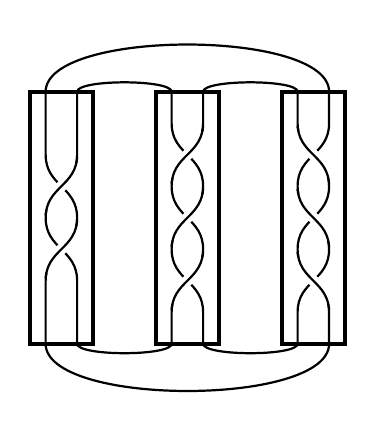
\begin{tikzpicture}[scale = 0.8]

\draw[ultra thick] (0, -0.5) rectangle (1, 3.5);
\draw[ultra thick] (2, -0.5) rectangle (3, 3.5);
\draw[ultra thick] (4, -0.5) rectangle (5, 3.5);

\begin{knot}[clip width = 5, flip crossing/.list={2, 4, 6, 8}]
\strand[thick] (0.25, -0.5) -- (0.25, 0.5) .. controls +(0, 0.5) and +(0, -0.5) .. (0.75, 1.5) .. controls +(0, 0.5) and +(0, -0.5) .. (0.25, 2.5) -- (0.25, 3.5);

\strand[thick] (0.75, -0.5) -- (0.75, 0.5) .. controls +(0, 0.5) and +(0, -0.5) .. (0.25, 1.5) .. controls +(0, 0.5) and +(0, -0.5) .. (0.75, 2.5) -- (0.75, 3.5);


\strand[thick] (2.25, -0.5) -- (2.25, 0) .. controls +(0, 0.5) and +(0, -0.5) .. (2.75, 1) .. controls +(0, 0.5) and +(0, -0.5) .. (2.25, 2) .. controls +(0, 0.5) and +(0, -0.5) .. (2.75, 3) -- (2.75, 3.5);

\strand[thick] (2.75, -0.5) -- (2.75, 0) .. controls +(0, 0.5) and +(0, -0.5) .. (2.25, 1) .. controls +(0, 0.5) and +(0, -0.5) .. (2.75, 2) .. controls +(0, 0.5) and +(0, -0.5) .. (2.25, 3) -- (2.25, 3.5);



\strand[thick] (4.25, -0.5) -- (4.25, 0) .. controls +(0, 0.5) and +(0, -0.5) .. (4.75, 1) .. controls +(0, 0.5) and +(0, -0.5) .. (4.25, 2) .. controls +(0, 0.5) and +(0, -0.5) .. (4.75, 3) -- (4.75, 3.5);

\strand[thick] (4.75, -0.5) -- (4.75, 0) .. controls +(0, 0.5) and +(0, -0.5) .. (4.25, 1) .. controls +(0, 0.5) and +(0, -0.5) .. (4.75, 2) .. controls +(0, 0.5) and +(0, -0.5) .. (4.25, 3) -- (4.25, 3.5);

\strand[thick] (0.75, -0.5) .. controls +(0, -0.2) and +(0, -0.2) .. (2.25, -0.5);
\strand[thick] (2.75, -0.5) .. controls +(0, -0.2) and +(0, -0.2) .. (4.25, -0.5);
\strand[thick] (0.25, -0.5) .. controls +(0, -1) and +(0, -1) .. (4.75, -0.5);


\strand[thick] (0.75, 3.5) .. controls +(0, 0.2) and +(0, 0.2) .. (2.25, 3.5);
\strand[thick] (2.75, 3.5) .. controls +(0, 0.2) and +(0, 0.2) .. (4.25, 3.5);
\strand[thick] (0.25, 3.5) .. controls +(0, 1) and +(0, 1) .. (4.75, 3.5);


\end{knot}
\end{tikzpicture}
\caption{$P(2, 3, -3)$}
\end{minipage}
\end{figure}
\end{example}


%TODO define this better
For two knots $K$ and $K'$ define their \textit{connected sum} $K\#K'$ to be the knot obtained by connecting the ends of the knots with short intervals removed.


%TODO
\begin{figure}[h]
\centering
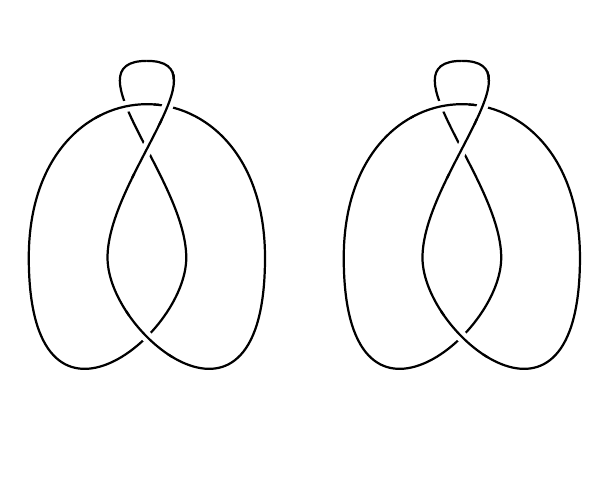
\begin{tikzpicture}
\begin{knot}[consider self intersections = true, ignore endpoint intersections=false, clip width = 5]
\strand[thick] (0, 1.5) .. controls +(1, 0) and +(0, 1) .. (-0.5, -1) .. controls +(0, -1) and +(0, -2.6) .. (1.5, -1) .. controls +(0, 2.6) and +(0, 2.6) .. (-1.5, -1) .. controls +(0, -2.6) and +(0, -1) .. (0.5, -1) .. controls +(0, 1) and +(-1, 0) .. (0, 1.5);


\strand[thick] (4, 1.5) .. controls +(1, 0) and +(0, 1) .. (3.5, -1) .. controls +(0, -1) and +(0, -2.6) .. (5.5, -1) .. controls +(0, 2.6) and +(0, 2.6) .. (2.5, -1) .. controls +(0, -2.6) and +(0, -1) .. (4.5, -1) .. controls +(0, 1) and +(-1, 0) .. (4, 1.5);

\end{knot}
\end{tikzpicture}
\caption{The connected sum of two trefoils}
\label{fig:connected-sum}
\end{figure}

\subsubsection{The Bridge Index}\label{subsubsec:bridge-index}
Let $L \subset S^3$ be a link. The minimal number of local maxima of a smooth function $S^3 \rightarrow \mathbb{R}$ restricted to $L$ is called the \textit{bridge index} of $L$ and referred to as $\text{bi } L$.

This can be diagrammatically characterized in the following way. Let $D$ be a diagram of $L$. An \textit{arc} in $D$ is a segment of $D$ beginning and ending with an undercrossing, containing no undercrossings in between. A \textit{bridge} of $D$ is an arc of $D$ that contains at least one overcrossing.

\begin{proposition}
The bridge index of a link $L \subset S^3$ is equal to the number of bridges in a diagram $D$ of $L$, minimized over all diagrams.
\end{proposition}

%TODO prove or cite

\begin{proposition}\label{prop:bridge-index-connected-sum}
Let $K$ and $K'$ be knots. Then $\textup{bi } K\#K' = \textup{bi } K + \textup{bi }K' - 1$.
\end{proposition}

\subsubsection{The Link Group}\label{subsubsec:the_knot_group}
%The Wirtinger algorithm and why the abelianization is isomorphic to the integers.

The \textit{link group} of a link $L \subset S^3$ is $\pi(L) = \pi_1(S^3 \setminus L)$. If $L$ is a knot $K$ then the link group $\pi(K)$ is referred to as its \textit{knot group}.

The knot group essentially classifies all knots, in that if two knots have isomorphic knot groups then they are equivalent. Be warned that this is no longer true for links. This suggests that studying the knot group might be just as good as studying knots themselves.

We will now describe an algorithm that computes the link group of an oriented link. Let $L \subset S^3$ be a link and let $D$ be any diagram of $L$. Let $S = \{m_1, \dots, m_k\}$ be the set of diagram meridians, oriented from right to left. A meridian $m_i$ should be interpreted at as the meridian starting at the reader's eye, passing under the arc and going back to the reader's eye without any detour.

Having assigned a generator to every crossing, we now assign a relator $r$ at any crossing, as described in Figure \ref{fig:wirtinger-relations}.

\begin{figure}[h]
\centering
\begin{minipage}{.5\textwidth}
\centering
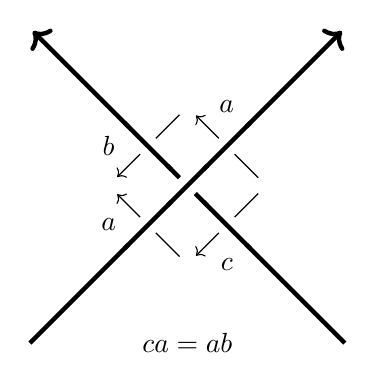
\begin{tikzpicture}
\begin{knot}[clip width = 5]
\strand[black, ultra thick, ->] (0, 0) -- (4, 4);
\strand[black, ultra thick, ->] (4, 0) -- (0, 4);

\strand[black, ->] (1.9, 1.1) -- (1.1, 1.9);
\strand[black, ->] (1.9, 2.9) -- (1.1, 2.1);
\strand[black, ->] (2.9, 2.1) -- (2.1, 2.9);
\strand[black, ->] (2.9, 1.9) -- (2.1, 1.1);

\node at (1, 1.5) {$a$};
\node at (1, 2.5) {$b$};
\node at (2.5, 3) {$a$};
\node at (2.5, 1) {$c$};

\node at (2, 0) {$ca = ab$};
\end{knot}
\end{tikzpicture}
\end{minipage}%
\begin{minipage}{.5\textwidth}
\centering
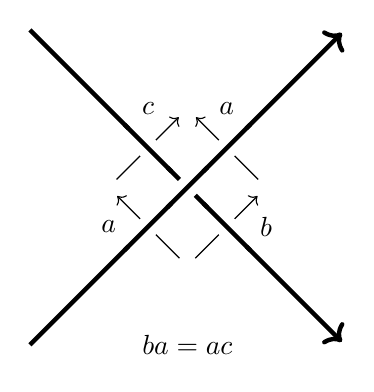
\begin{tikzpicture}
\begin{knot}[clip width = 5]
\strand[black, ultra thick, ->] (0, 0) -- (4, 4);
\strand[black, ultra thick, ->] (0, 4) -- (4, 0);

\strand[black, ->] (1.9, 1.1) -- (1.1, 1.9);
\strand[black, ->] (1.1, 2.1) -- (1.9, 2.9);
\strand[black, ->] (2.9, 2.1) -- (2.1, 2.9);
\strand[black, ->] (2.1, 1.1) -- (2.9, 1.9);

\node at (1, 1.5) {$a$};
\node at (1.5, 3) {$c$};
\node at (2.5, 3) {$a$};
\node at (3, 1.5) {$b$};

\node at (2, 0) {$ba = ac$};
\end{knot}
\end{tikzpicture}
\end{minipage}
\caption{Relations in the Wirtinger Presentation}
\label{fig:wirtinger-relations}
\end{figure}

The fact that the resulting presentation is actually a presentation for the link group of $L$ is a Seifert-van Kampen argument, elaborated upon for example in Rolfsen.
%TODO cite.

\subsubsection{The Meridional Rank}
%The definition, the meridional rank conjecture, partial results therein, comments about how complicated this is.


It turns out that one of the relations in the resulting presentation is redundant, and that it is always enough to only consider $n = \text{bi } L$ generators of $\pi(L)$ that are so-called \textit{meridians}, that is, curves that generate the first homology group $H_1(S^3 \setminus L)$. They can also be defined to be curves conjugate in $\pi(L)$ to a \textit{diagram meridian}, as indicated in Figure \ref{fig:diagram-meridian}.

\begin{figure}
\centering
\begin{tikzpicture}

\begin{knot}[clip width = 5, flip crossing = 2]
\strand[black, thick] (0, 0) -- (0, 4);
\strand (-1, 2) .. controls +(0, 0.5) and +(0, 0.5) .. (1, 2) .. controls +(0, -0.5) and +(0, -0.5) .. (-1, 2);
\end{knot}

\node at (0.8, 1.4) {$m$};

\end{tikzpicture}
\caption{A Diagram Merdian $m$}
\label{fig:diagram-meridian}
\end{figure} 

By definition, the \textit{meridional rank} of a link $L \subset S^3$ is the minimal number of meridians of $L$ needed to generate $\pi(L)$. We will the denote the meridional rank of $L$ by the symbol $\text{mr } L$. Thus, by the above remark we have that $\text{mr } L \leq \text{bi } L$. In fact, it is believed that this is actually an equality.

%TODO give credit
\begin{conjecture}[Meridional Rank Conjecture]
Let $L \subset S^3$ be a link. Then the meridional rank of $L$ is equal to its bridge index.
\end{conjecture}

\subsection{Group Theory}
\subsubsection{Normal Subgroups}
Recall that a \textit{group} is a set $G$ with an associative multiplication $\cdot$ such that there exists a neutral element $e$ satisfying $eg = g = ge$ for all $g \in G$, and for any $g \in G$ there exists a multiplicative inverse $g^{-1}$ satisfying $gg^{-1} = e = g^{-1}g$. A \textit{subgroup} of a group is a subset $H$ of $G$ that is itself a group with neutral element $e$.

A subgroup $N$ of $G$ is \textit{normal} if for any $g \in G$ we have that $gNg^{-1} = N$. Recall that the quotient $G/N$ is a group if and only if $N$ is a normal subgroup of $G$. Recall also that the intersection of arbitrarily many normal subgroups is also a normal subgroup of $G$. Because of this, for any subset $S \subset G$ we can define its \textit{normal closure} $\langle \langle S \rangle \rangle$ to be the smallest normal subgroup of $G$ containing $S$.

The \textit{commutator subgroup} of $G$ is the normal closure of the set $S$ of \textit{commutators}, i.e., elements of the form $aba^{-1}b^{-1}$ for $a, b \in G$. We write $[G, G]$ for the commutator subgroup. Then, the \textit{abelianization} of $G$ is the group $G^{\text{ab}} = G / [G, G]$.

\subsubsection{Presentations}
A group $F$ is called \textit{free} over a set $S$ if for any group $G$, any map $S \rightarrow G$ extends uniquely to a homomorphism $F \rightarrow G$ as in the following diagram:

\begin{figure}[ht]
\centering
\begin{tikzcd}
S \arrow[r, hook] \arrow[dr] & F \arrow[d, dashrightarrow] \\
& G 
\end{tikzcd}
\end{figure}

The property of being free over a set $S$ determines the group up to isomorphism.
A \textit{presentation} $\langle S, R \rangle$ is the group $F/\langle \langle R \rangle \rangle$, where $F$ is a free group over the \textit{generating set} $S$ subjects to the \textit{relations} $R \subset F$.

Presentations arise naturally in many situations, most notably when applying the Seifert-van Kampen theorem, compare \cite{hatcher2002}. This makes them a very useful tool with one important drawback: they are notoriously hard to handle. A particular symptom of this is the following problem.

\begin{problem}[Word Problem]
Let $G = \langle S \; | \; R \rangle$.
Given a word $w$ in the free group over $S$, does $w$ represent the identity in $G$?
\end{problem}

Innocent as it seems, the word problem is actually unsolvable in general. That is, there exist presentations $\langle S \; | \; R \rangle$ for which there is no algorithm that is guaranteed to give the right answer to the word problem in a finite amount of time.

The following other problem for which there is no algorithm solution annihilates the usefulness of the fundamental group of a link complement to distinguish links completely.

\begin{problem}[Isomorphism Problem]
Given two presentations $\langle S \; | \; R \rangle $ and $ \langle S' \; | \; R' \rangle$, do they present isomorphic groups?
\end{problem}

Although both these problems are unsolvable in general, there exists a rich class of groups for which they are: the Coxeter groups.

\subsection{Coxeter Groups}\label{sub:coxeter_groups}
Let $S$ be a finite set and let $M = (m_{st})$ be an $S \times S$ matrix with coefficients in the set $\mathbb{N} \cup \{\infty\}$ satisfying $m_{ss} = 1$ for all $s \in S$, and $m_{st} \geq 2$ if $s \ne t$. Such a matrix is called a \textit{Coxeter matrix}. Consider the group presentation
$$W(M) = \langle S \; | \; (st)^{m_{st}} = 1 \text{ for } s,t\in S \rangle,$$
where we do not include equations of the form $(st)^\infty = 1$.
Then the group $W(M)$ is called the \textit{Coxeter group} corresponding to $M$. The tuple $(W(M),S)$ is called a \textit{Coxeter system} and the cardinality $\#S$ is referred to as its \textit{rank}. Since for us Coxeter groups always arise with a generating set, we blur the distinction between Coxeter groups and Coxeter systems.

Another way to encode the coefficients $m_{st}$ is to use them as weights in weighted undirected graphs, so-called \textit{Coxeter graphs}. In this case, the nodes of the graph are the generators, and the weight between the nodes $s$ and $t$ is $m_{st}$. The following shorthand notations are very common: If $m_{st} = 2$, then the edge between $s$ and $t$ is omitted and if $m_{st} = 3$, then the weight on the edge between $s$ and $t$ is omitted.

\begin{example}[Dihedral Groups]
The symmetry group of a regular $n$-gon is called the \textit{dihedral group} of order $2n$, denoted by the symbol $D_n$. This group is generated by two reflections $s, t$ whose composition is a rotation by an angle of~$2\pi/n$. This is used to show that $D_n$ is isomorphic to the Coxeter group
$$W = \langle s, t \; | \; (st)^n = s^2 = t^2 = 1 \rangle.$$
Thus, Coxeter groups on two generators whose product has finite order are dihedral groups.

This observation is often used to motivate the introduction of one more dihedral group, the so-called \textit{infinite dihedral group} with presentation
$$\langle s, t \; | \; s^2 = t^2 = 1 \rangle$$
corresponding to the matrix
$$M = \left(\begin{matrix}
1 & \infty \\
\infty & 1
\end{matrix}\right).$$
\end{example}

\subsubsection{The Reflection Representation}
A well-known construction leading to an easy solution of the word-problem for Coxeter groups and also helping in adapting a geometric viewpoint to the study of Coxeter groups is a faithful representation of any Coxeter group where its generating sets acts as a set of reflections with respect to a (possibly degenerate) bilinear form.

Let $(W,S)$ be a Coxeter system, and let $n = \#S$. Then we consider the bilinear form on $\mathbb{R}^n$ given by the matrix $B = (b_{st})$ with entries $b_{ij} = -\cos \pi/n$. 
For $s \in S$ let $\rho_s$ be the \textit{reflection} with respect to $B$ with root $e_s \in \mathbb{R}^n$ given by the formula
$$ \rho_s(x) = x - 2B(x, e_s)e_s,$$
where $x \in \mathbb{R}^n$.

\begin{proposition}
Let $(W,S)$ be a Coxeter system and let $s, t \in S$. Then the reflections $\rho_s$ and $\rho_t$ satisfy $(\rho_s \rho_t)^{m_{st}} = 1$.
\end{proposition}

%TODO proof

This shows that the map $s \mapsto \rho_s$ induces a representation of $W$, called the \textit{reflection representation} of $W$.

\begin{theorem}
The reflection representation is faithful.
\end{theorem}

\subsubsection{The Word Problem}
In this section we study an alternative solution to the word problem in Coxeter groups due to Tits. %TODO cite
\begin{notation}
Let $W$ be a Coxeter group with generating set $S$ and Coxeter matrix $M = (m_{st})$. Then we agree on the convention that
$$(st)^{m_{st}/2} =  \begin{cases}
(st)^k & \text{ if } m_{st} = 2k, \\
(st)^ls & \text{ if } m_{st} = 2l + 1.
\end{cases}$$
E.g., if $m_{st}=5$ we write $(st)^{5/2} = ststs$. 
\end{notation}

%TODO cite properly
\begin{theorem}[Tits]\label{thm:word-problem}
Let $F$ be the free monoid generated by the set $S$. Suppose the word $w \in F$ represents the trivial element in a Coxeter group $W$ with generating set $S$ and Coxeter matrix $M = (m_{st})$. Then there is a sequence of moves of the following two types carrying $w$ to the empty word.

\begin{enumerate}[\textup{(}i\textup{)}]
\item removing occurrences of $s^2$ from $w$ for $s \in S$.
\item replacing occurrences of $(st)^{m_{st}/2}$ by $(ts)^{m_{st}/2}$ for $s, t \in S$.
\end{enumerate}

\end{theorem}

\newpage

\section{Some Algorithms}
We describe in this section in some detail how to implement some of the strategies we more or less vaguely described in the above sections.
\subsection{General Knot Theory}
\subsubsection{Gauss Codes}
There are numerous ways to represent a link numerically on a computer. The oldest way, which is absolutely sufficient for our purposes, is to represent them as (unoriented, weighted) Gauss codes. Let $D$ be a diagram of any link $L$. Number the crossings of $D$ in an arbitrary way. Now for each component $K_i \subset L$ let $C_i$ be the tuple obtained by tracing along the knot $K_i$ and at each crossing $k$ add the number $k$ to $C_i$ if $k$ is an overcrossing, and $-k$ otherwise.
Then, the \textit{Gauss code} of $L$ is the set $\{C_1, \dots, C_m\}$, where $m$ is the number of components of $L$.

\begin{examples}
The Gauss code of the trefoil knot, which can also be described as the $(2,3)$-torus knot, is $\{(-1, 2, -3, 1, -2, 3)\}$. The Gauss code of the Hopf link, which is also the $(1, 2)$-torus knot, is $\{(1, -2), (-1, 2)\}$. The numbering of crossings used can be seen in Figure \ref{fig:numbered-crossings}.

\begin{figure}[ht]
\label{fig:numbered-crossings}
\centering
\begin{minipage}{.5\textwidth}
 \centering
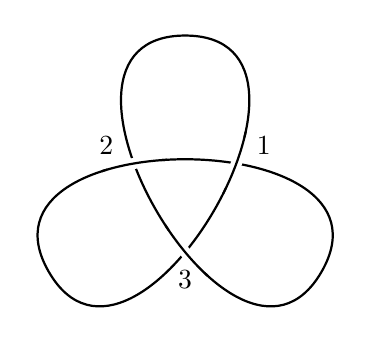
\begin{tikzpicture}
\clip (-2, -1.8) rectangle (2,2.1);
\begin{knot}[clip width = 5, consider self intersections = true, flip crossing = 2]

\strand[black, thick] (0,2) .. controls +(2.2,0) and +(120:-2.2) .. (210:2) .. controls +(120:2.2) and +(60:2.2) .. (-30:2) .. controls +(60:-2.2) and +(-2.2,0) .. (0,2);

\node at (1,0.6) {1};
\node at (-1, 0.6) {2};
\node at (0, -1.1) {3};

\end{knot}
\end{tikzpicture}
\end{minipage}%
\begin{minipage}{.5\textwidth}
 \centering
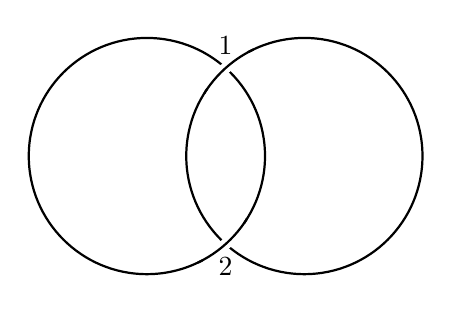
\begin{tikzpicture}


\begin{knot}[clip width = 5, flip crossing=2]

\strand[black, thick] (1,0) circle[radius=1.5];
\strand[black, thick] (-1,0) circle[radius=1.5];

\node at (0, 1.4) {1};
\node at (0, -1.4) {2};
\end{knot}
\end{tikzpicture}
\end{minipage}

\caption{Numbered crossings of the trefoil knot (left) and the Hopf link (right)}
\end{figure}


\end{examples}

Some care should be taken when defining Gauss codes in the way we do, since Gauss codes for knots do not capture the orientation of a knot. The situation is even worse for links. In other words, Gauss codes do not uniquely determine the knot or link in question. But since if two links have equivalent Gauss codes they will have the same fundamental group, we will not further address this matter.

\subsubsection{The Wirtinger Algorithm}
In order to have a more concrete idea how to implement the Wirtinger algorithm, we first have to see how we can extract information from the Gauss code $G$ of a link $L$. A simple example is the following. An \textit{arc} in a Gauss code $G$ is a subtuple of the tuple $C$ corresponding to a component $K$ of $L$ of the form $$A = (-a, x_1, \dots, x_d, -b),$$ where all of the numbers $a, b, x_1, \dots, x_d$ are positive. This corresponds to a line in the diagram of $L$. In this way, every crossing can be interpreted to be part of a unique arc that has this crossing as an overcrossing, and a part of two arcs that have this crossing as an undercrossing. Note that, e.g., in the case of the Hopf link, these two arcs may coincide.

Now that we have settled how to represent an arc of a Gauss code, let us consider what information should be available from the representation of a crossing. Of course, one of the numbers $k$ present in the Gauss code would be enough to specify the crossing, but for us it will be more useful to encode crossings in the following way. Notice that at each crossing, three arcs meet. One of them is the over-arc $A$, and two others, say $B$ and $C$, are under-arcs. Then we write $c = (A, B, C)$ for this crossing.

In the pseudocode of Algorithm \ref{alg:wirtinger1} we present a basic version of the Wirtinger algorithm. This version assigns to each crossing $c$ a relation in the symbols corresponding to arcs of the Gauss code, written $c.A, c.B,$ and $c.C$.

\begin{algorithm}\label{alg:wirtinger1}
\KwData{A Gauss code $G$}
\KwResult{A presentation of the knot group of $G$}
compute the variables \textit{arcs} and \textit{crossings}\;
$\textit{rels} \leftarrow \emptyset$\;
\For {$c$ in \textit{crossings}}{
	$\textit{rels} \leftarrow \textit{rels} \cup \{c.A \cdot c.B \cdot c.A^{-1} \cdot c.C^{-1}\}$
}
remove one relation from \textit{rels}\;
\Return $\langle \textit{arcs} \; | \; \textit{rels}\rangle$\;
\caption{The Wirtinger Algorithm, Version 1}
\end{algorithm}

\begin{algorithm}\label{alg:good-generating-sets}
\KwData{A Gauss code $G$}
\KwResult{All sets of generators of minimal size}
\caption{Finding minimal generating sets}
compute the variables \textit{arcs} and \textit{crossings}\;
$\textit{generatingSets} \leftarrow \emptyset$\;
\For{$\textit{rank} = 1 \dots \#\textit{crossings}$}{
$\textit{combs} \leftarrow$ all combinations of \textit{rank} arcs\;
\For{comb in combs}{
$\textit{marked} \leftarrow \textit{comb}$\;
$\textit{markedSomething} \leftarrow $ True\;
\While{\textit{markedSomething}}{
$\textit{markedSomething} \leftarrow $ False\;
\For{c in crossings}{
\If{$c.A$ in marked and $c.B$ in marked}{
\If{$c.C$ not in marked}{
$\textit{marked} \leftarrow \textit{marked} \cup \{ c.C \} $\;
$\textit{markedSomething} \leftarrow $ True\;}}
\If{$c.A$ in marked and $c.C$ in marked}{
\If{$c.B$ not in marked}{
$\textit{marked} \leftarrow \textit{marked} \cup \{ c.B\} $\;
$\textit{markedSomething} \leftarrow $ True\;}}}}
\If{$\textit{marked} = \textit{arcs}$}{
$\textit{generatingSets} \leftarrow \textit{generatingSets} \cup comb$\;}}
\If{$\textit{generatingSets} \ne \emptyset$}{
\Return $\textit{generatingSets}$}}
\end{algorithm}


Because of our approach of finding Coxeter quotients in \ref{subsec:coxeter_quotients_algorithms}, this sort of presentation will not be of much use to us since it involves too many generators in general. We are aiming for a presentation involving only as many generators as the bridge index of the corresponding link.

A solution to identifying reasonably sized sets of generators is given in Algorithm \ref{alg:good-generating-sets}. At the time of writing it is an open question whether this algorithm actually produces generating sets of size the bridge index, but in practice it works really well for small knots, i.e., less than 10 crossings.

From Algorithm \ref{alg:good-generating-sets} one can pretty much infer how the second version of Wirtinger will go: instead of marking, we just express the arcs as product of the already expressed arcs. In this way we obtain a list of presentations, all with the same number of generators, which is most likely the bridge index of the link.

\subsection{Coxeter Quotients}\label{subsec:coxeter_quotients_algorithms}
\subsubsection{Obvious Visible Coxeter Quotients}
Let $D$ be a diagram of a link $L$. Ideally, we would like an algorithm producing from the Gauss code corresponding to $D$ a list of all surjective homomorphisms onto Coxeter groups. Since for now there do not exist much better techniques than brute-forcing your way into those quotients, this is not realistic even for a fixed infinite Coxeter group. So we need to settle for an even more specific class of Coxeter quotients.

Let $D$ be a Gauss code. Then a generating set of diagram meridians is \textit{obvious} if \ref{alg:good-generating-sets} detects that they are a generating set. Moreover, a Coxeter quotient is visible if for all generators $s \in S$ there exist diagram meridians in the preimage in the knot group.

\subsubsection{Finding Quotients}
After having solved the word problem in Coxeter groups it is rather straightforward to find obvious visible Coxeter quotients, as can be seen in the pseudocode of Algorithm \ref{alg:obvious-visible-coxeter-quotients}.
\begin{algorithm}\label{alg:obvious-visible-coxeter-quotients}
\caption{Finding obvious visible Coxeter quotients}
\KwData{A Wirtinger presentation $\langle \textit{gens} \; | \; \textit{rels} \, \rangle$}
\KwResult{All matrices corresponding to obvious visible Coxeter quotients}
$n \leftarrow \#\textit{gens}$\;
$\textit{max} \leftarrow $ the length of the longest relator\;
$\textit{quotients} \leftarrow \emptyset$\;
\textit{matrices} $ \leftarrow $ all $n \times n$-matrices with entries in $\{1, \dots, \textit{max}, \infty \}$\;
\For{\textit{matrix} in matrices}{
\If{all rel in rels hold in the Coxeter group $W(\textit{matrix})$}{
$\textit{quotients} \leftarrow \textit{quotients} \cup \{matrix\}$}}
\Return \textit{quotients}
\end{algorithm}

The justification for not considering entries less than the length of the longest relator lies in the fact that Tits' solution to the word problem does not increase word length, see Theorem \ref{thm:word-problem}. 
\newpage

\bibliography{biblio}
\bibliographystyle{plain}

\end{document}